\section{Programstruktur}



\begin{figure}[h]
\centering
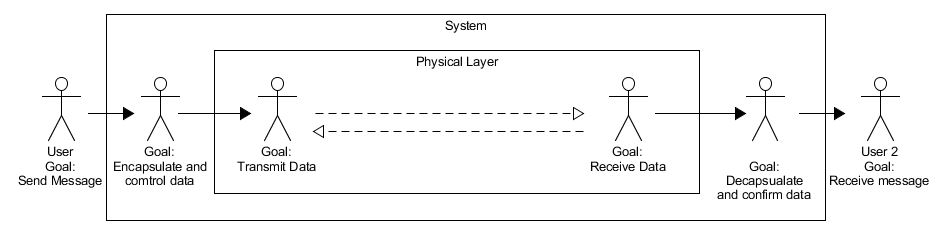
\includegraphics[scale=0.5]{Billeder/ProgramOpbygning1.JPG}
\caption{Jeg kan se at det virker, så det virker}
\label{fig:Blokdiagram}
\end{figure}

som det kan ses i figur \ref{fig:Blokdiagram} er alt fedt. 


\textbf{klade}
formål med dette afsnit: Her skal der dannes et overblik over projektet
Hvordan nåede vi frem til opbygningen af projektet\\

-Vis klassediagram (blok diagram)\\
-klasse diagrammet anvendt til dette proke t

Indledning 
kommer Direkte fra primær og sekundære krav. 
produktet skal formes
der tages udgangspunkt i internetstrukturen
Hvordan forvæntes de forskellige “sorte kasser” at arbejde sammen (grænse flader)

det viste klassediagram er et udkast til programmet, og kan derfor ændre sig efter behov gennem projektet. nedenstående.

Jævnføre projektoplæget skal der anvendes en lagsopdelt arkitektur. 
Inspireret af internet strukturen

Hvordan skal en domænemodel opbygges for at sikre denne karakteristik. 
Det er her Software udviklingsprincipper kommer ind i billedet


\subsection{UML – Ansvarsfordeling til klasser}
-Udpenslende forklaring af ansvarsfordeling og programstruktur.  